\documentclass{article}

\usepackage[english]{babel}
\usepackage{tgtermes}
\usepackage{xcolor}
\usepackage{pagecolor}
\usepackage{hyperref}
\usepackage{graphicx}
\usepackage[labelformat=empty]{caption} 


\definecolor{draculabg}      {RGB} {25,   25,   25}
\definecolor{draculacl}      {RGB} {68,   71,   90}
\definecolor{draculafg}      {RGB} {248,  248,  242}
\definecolor{draculacomment} {RGB} {98,   114,  164}
\definecolor{draculacyan}    {RGB} {139,  233,  253}
\definecolor{draculagreen}   {RGB} {80,   250,  123}
\definecolor{draculaorange}  {RGB} {255,  184,  108}
\definecolor{draculapink}    {RGB} {255,  121,  198}
\definecolor{draculapurple}  {RGB} {189,  147,  249}
\definecolor{draculared}     {RGB} {216,  47,   49}
\definecolor{draculayellow}  {RGB} {241,  250,  140}
\definecolor{draculablue}  {RGB} {36,  85,  151}

\pagecolor{draculabg}
\color{draculafg}

\nocite{*}

\title{\textbf{Aldone}}
\author{Fausto Zamparelli, Daniel Falbo}
\date{May 30, 2024}

\hypersetup{
colorlinks=true,
linkcolor=draculapurple,
citecolor=draculapurple,
urlcolor=draculapurple,
pdftitle={Aldone},
pdfpagemode=FullScreen,
}

\begin{document}

\maketitle

\section*{\color{draculagreen}Introduction}
Aldone as in "AI-Done" is our own way to streamline task management and to maximize productivity. This product is just a proof of concept but already can do so much to help you in your day to day tasks.

\subsection*{\color{draculayellow}{Functionality}}
What can Aldone do for you, you may ask...

Aldone can be your interactive daily task logger controlled only by your voice. Our vision is an assistant you can talk to and then make questions to, for the sole purpose of helping you achieve tasks faster in a world full of distraction and where time is more and more valuable.

Aldone, is web based for now. After a log-in you will be able to speak to it to add tasks you need to accomplish or make questions about todos you told him earlier, but it doesn't end here: you could ask him for example to split a task in sub-tasks to approximate how long a task will take and  much more... The possibilities are endless. We implemented also a neat feature from a highly requested functionality especially from Italian moms. We added to Aldone the functionality to be able to detect fully by himself weather you are asking him to add something to your own grocery list in order to make it really easy to then retrieve everything you may have added through the week. The coolest thing is that once you will come home from the supermarket with tired legs and arms from carrying bags, you won't have to manually remove everything from this digital grocery list but you can use your phone camera to detect what foods you actually bought and then Aldone will remove them for you. It is very simple and useful in the case you didn't actually buy everything that was on the list let's say for example that a product wasn't available that day, Aldone will then keep it in the list so that you won't forget to buy it the next time. 

\newpage

\section*{\color{draculagreen}Method} 
\begin{figure}[htbp]
\centering
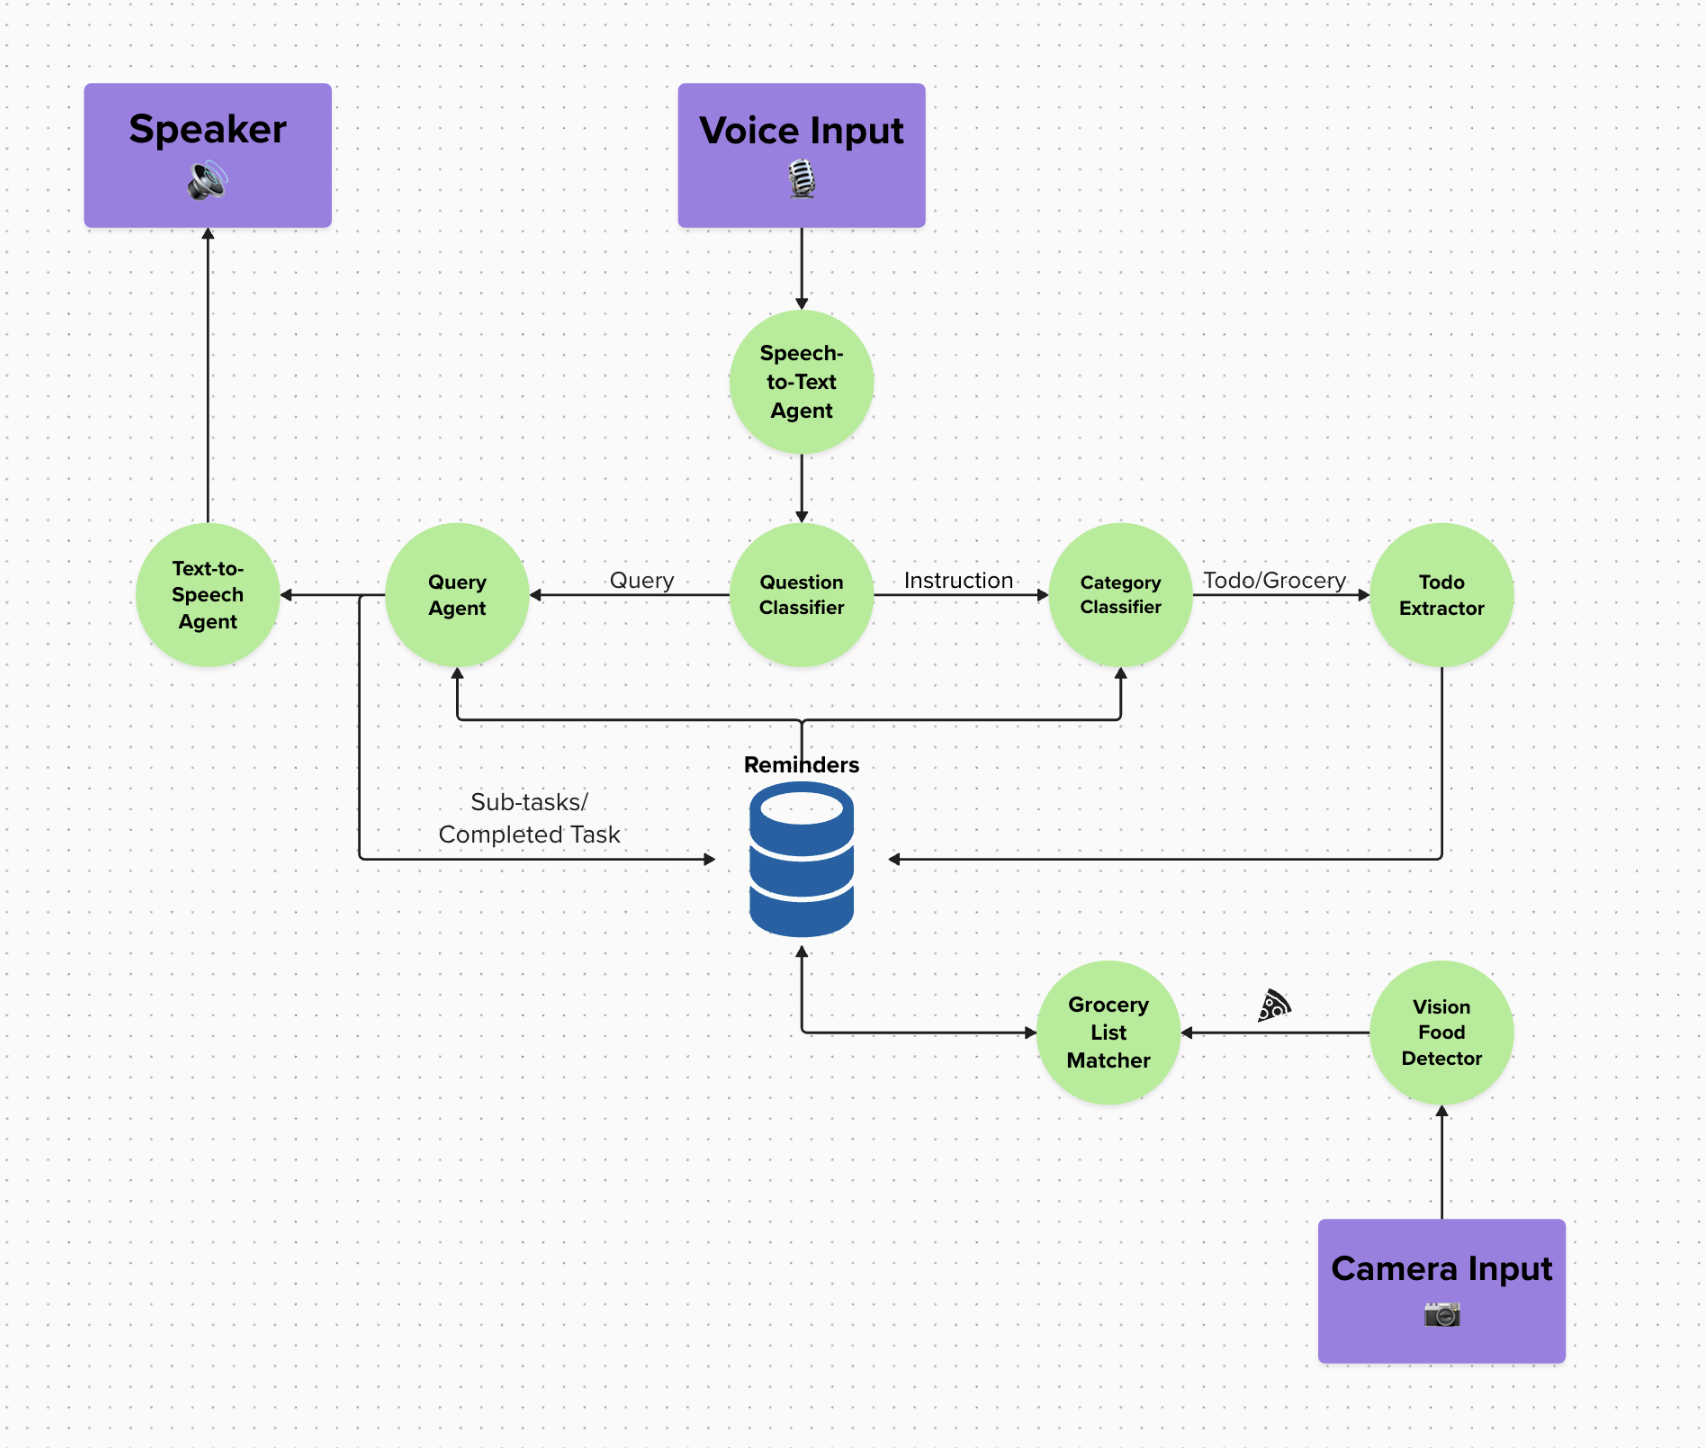
\includegraphics[width=\textwidth]{diagram.png}
\caption{\small Visual representation of the agents that make up Aldone}
\end{figure}

As we can see Aldone was created by splitting its functionality into various agents that cooperate with each others. In order to fully understand how Aldone works under the hood it is best to understand the functionality of these agents. Let's work our way thorough the graph from top to bottom following the arrows:

\subsection*{\color{draculayellow}Speech-to-Text Agent}
As mentioned before Aldone is a web app that uses Next.js, for this reason in order to make speech to text as fast as possible while still being reliable we choose to use the \href{https://developer.chrome.com/blog/voice-driven-web-apps-introduction-to-the-web-speech-api}{browser API} to handle the speech-to-text since nowadays is pretty much supported in every commonly used browsers.

\subsection*{\color{draculayellow}Question Classifier}
The question classifier in case is a folder where we used pytorch to create a neural network that is able to detect weather each phrase the user says to our Speech-To-Text agent is a query or an instruction. This is crucial in order to be able to keep traversing the agents in our graph. We needed a way in fact to be able to make Aldone recognize weather the user is asking something to him in which case we would pass the query to the General Agent which will be able to respond to the query regarding todos or weather the phrase is an instruction in this case the actions needed should be to add a todo inside the database which will be handled by the Category classifier going forward.

In the folder is present:
\begin{itemize}
 \item \texttt{nndata.json}: this is the dataset used to train the model it contains 150 prompts inside a json file where each entry is a table with a text and a label (1 if it is a query, 0 if it is a statement)
  \item \texttt{nntraining.py}:
  \begin{enumerate}
    \item \textit{Data Loading}: Loads the data from a JSON file. Each item in the data is a dictionary with a "text" field and a "label" field.
    \item \textit{Data Splitting}: Splits the data into training, validation, and test sets using stratified sampling.
    \item \textit{Text Vectorization}: Converts the text into a numerical representation using the `CountVectorizer` from `sklearn`.
    \item \textit{Data Conversion}: Converts the data and labels into PyTorch tensors, which are used to create a `DataLoader` for each set.
    \item \textit{Model Definition}: Defines a `TextClassifier` model, which is a simple feed-forward neural network with one hidden layer and a sigmoid activation function on the output layer.
    \item \textit{Training Loop}: Trains the model for a specified number of epochs. In each epoch, it computes the loss and updates the model's parameters. It also evaluates the model on the validation data and prints the training and validation loss.
    \item \textit{Model Evaluation}: Evaluates the model on the test data and prints the accuracy.
    \item \textit{Model Output}: labelmodel.pth (the trained model) and labelvectorizer.joblib (the fitted vectorizer), which are both used in the `nnlabeler.py` script.
  \end{enumerate}
  \item \texttt{nnlabeler.py}: responsible for applying the trained model to new text data
  \begin{enumerate}
    \item \textit{Model and Vectorizer Loading}: Loads the trained model and the vectorizer from disk.
    \item \textit{Text Vectorization}: Converts the input text into a numerical representation using the loaded vectorizer.
    \item \textit{Data Conversion}: Converts the vectorized text into a PyTorch tensor.
    \item \textit{Model Application}: Passes the tensor through the model to get the predicted probability of the text being a question.
    \item \textit{Prediction}: Rounds the predicted probability to get the predicted label (1 for question, 0 for statement).
    \item \textit{Query Function}: Provides a function that returns `True` if the text is predicted to be a question and `False` otherwise.
    \item \textit{Command-Line Interface}: If the script is run from the command line with a text argument, it prints the predicted label for the text.
  \end{enumerate}
\end{itemize}

**add image of the accuracy**

\section*{If the phrase is an Instruction}
\subsection*{\color{draculayellow}Category Classifier}

\subsection*{\color{draculayellow}Todo Extractor}

[Confusion Matrix here]

\subsection*{\color{draculayellow}Vision Food Detector}

We first asked the LLM model to give us the entire updated grocery list object, but empirically it often made errors. What we ended up doing is asking the LLM model for indices of the grocery list that were updated, and then we updated the grocery list object ourselves. This way, we could ensure that the grocery list object was updated correctly.

\subsection*{\color{draculayellow}Grocery List Matcher}

\section*{If the phrase is an Query}

\subsection*{\color{draculayellow}General Agent}

\subsection*{\color{draculayellow}Text-to-Speech Agent}

\section*{\color{draculagreen}Results}

\subsection*{\color{draculagreen}Glue Orchestration}

\section*{\color{draculagreen}Source of inspiration}

[1] \href{https://humane.com/media/cosmos-an-operating-system-for-the-ai-era}{Cosmos: An Operating System for the AI Era} \newline
[2] aiXplain

\end{document}
